% ============================================================================
%  Concentrate or Spread? — DiffSoup topology paper (DRAFT SKELETON)
%  Build:  cd paper && latexmk -pdf main.tex      (requires a TeX install)
%  NOTE: this skeleton was NOT compiled by its author tool (no TeX toolchain on
%  the authoring machine). Run latexmk yourself; see ../NOTES_FOR_AUTHOR.md.
%
%  GROUNDING CONTRACT (enforced throughout):
%   * every numeric result carries a "% src: <file>" comment naming the results
%     file it was read from. No number appears without one.
%   * citations are REAL (refs.bib, filled + verified against publisher/arXiv
%     pages 2026-07-03; page numbers omitted where unverifiable, not guessed).
%   * the dimensional-crossover section (5c) is a SCAFFOLD: setup prose + \TODO
%     markers only, no results (per the author's R3).
%   * claim strength is capped at the abstract (R5).
% ============================================================================
\documentclass[11pt]{article}

\usepackage[utf8]{inputenc}
\usepackage[T1]{fontenc}
\usepackage[margin=1in]{geometry}
\usepackage{graphicx}
\usepackage{booktabs}
\usepackage{multirow}
\usepackage{amsmath,amssymb}
\usepackage{xcolor}
\usepackage[numbers,sort&compress]{natbib} % sorted+compressed [1-3] citation brackets
\usepackage{hyperref}
\hypersetup{colorlinks=true, linkcolor=blue, citecolor=blue, urlcolor=blue}
\graphicspath{{figures/}}

% Visible marker for anything a human must fill (R4). Greppable as "TODO".
\newcommand{\TODO}[1]{\textcolor{red}{\textbf{[\,TODO: #1\,]}}}

% TODO(human): choose the venue style file and swap \documentclass accordingly.
% TITLE revised: dropped "The Dimensional Structure of Topological Priors" --- the
% dimensional-crossover hypothesis was REFUTED by the B4 data (a spread prior
% dominates at every dimension). Author may prefer the assertive
% "Spread, Don't Concentrate: ..." (R4: your call).
\title{Concentrate or Spread? Shaping Topological Resampling Priors\\
       for Differentiable Triangle-Soup Reconstruction}
% Shared affiliation, both authors. TODO(human): add emails / corresponding-author
% mark, and reformat to the venue's author block when the document class is swapped.
\author{Viritphon Chongpermwattanapol \qquad Pizzanu Kanongchaiyos\\[4pt]
  Department of Computer Engineering, Faculty of Engineering,\\
  Chulalongkorn University, Bangkok, Thailand}
\date{\today}

\begin{document}
\maketitle

% ----------------------------------------------------------------------------
% ABSTRACT --- data-supported thesis (reconciliation option A), CUT to <=250
% words in the 2026-07-03 mechanical pass: same claims, fewer words. Dropped to
% the body: per-shape percentages, sigma values, phantom-handle numerics, B1
% washout mechanics; one headline range (33--53%%) kept. Grounding unchanged:
%   blindness -> figures/summary.md ; 33--53%% + width-primary -> h2_unified/ ;
%   spread >= concentrate everywhere, loop cost -> crossover/ (+ report B5 arm).
% TODO(human): review the wording in your own voice; this is my draft, not yours.
% ----------------------------------------------------------------------------
\begin{abstract}
Differentiable rasterization reconstructs a 3D triangle soup from images by
following photometric gradients while periodically resampling triangles. We
first show this pipeline is topologically blind: Chamfer and Hausdorff
distances cannot separate reconstructions that differ in genus, connectivity,
or enclosed-void structure, while the bottleneck distance between persistence
diagrams can; a topological bias supplied at initialization is erased by the
first resampling step. Correct topology therefore requires in-loop guidance
and a persistence-based metric to detect it. We introduce topology-aware
adaptive resampling: a precomputed importance field that localizes the
target's persistent features and biases where new triangles respawn and which
are protected from pruning; budget-neutral, it reduces exactly to the baseline
when disabled. A single mass-preserving scale interpolates between a
\emph{concentrated} prior (importance piled on each feature's localized
death-simplex) and a \emph{spread} prior (the same mass over the feature's
support). We find no dimensional crossover: a spread prior is at least as good
as concentrating at every dimension and strictly better for voids and
loops---for enclosed voids it cuts bottleneck distance 33--53\% below the
baseline. The gain is carried by \emph{width} rather than topological
placement: a width-matched non-topological control recovers most of it,
leaving a small, shape-dependent residual for voids, a small cost on the loop,
and a null for components. The reason is that a feature's death-simplex is a
localized witness, not its full support, so the right bias spreads importance
over that support. The prescription: \emph{spread}, do not concentrate---the
caveat: the benefit comes from width, not topological targeting per se.
\end{abstract}

% ===== 1. Introduction (DRAFTABLE) ==========================================
\section{Introduction}
\label{sec:intro}

Differentiable rasterization optimizes an explicit 3D representation directly
against multi-view images by backpropagating a photometric loss through the
rasterizer~\cite{loper2014opendr,kato2018neural,liu2019softras,laine2020nvdiffrast}.
A \emph{triangle soup}---an unstructured collection of triangles
with no shared connectivity---is an attractive such representation: it is cheap
to render, places no manifold constraint on the geometry, and supports
\emph{adaptive resampling}, a periodic in-loop step that prunes
poorly-contributing triangles and respawns new ones to redistribute resolution
where the image residual demands it, in the spirit of the adaptive
densify-and-prune loops of explicit-primitive and mesh-evolution
pipelines~\cite{kerbl2023gaussians,held2025trianglesplatting,nicolet2021largesteps,palfinger2022remeshing}.
% NOTE: the DiffSoup renderer/trainer this instantiates is our own (unpublished)
% system; add its citation here once it is public.

Such pipelines are tuned to minimize geometric error, and geometric error is
exactly what they reduce. But geometry and \emph{topology} are different: a
reconstruction can be everywhere close to the target surface yet wrong in genus,
in the number of connected components, or in whether an enclosed void survives.
Our first contribution is to show that the standard pipeline is
\emph{topologically blind} in a precise, measurable sense. We construct matched
pairs of candidate reconstructions whose Chamfer distance to the ground truth is
\emph{equal by construction} but whose topology differs, and show that
Chamfer---and even Hausdorff---cannot separate them, whereas the
bottleneck distance between persistence diagrams can
(Section~\ref{sec:results-blindness}). We further observe that a topological
bias injected only at \emph{initialization} is erased: the first resampling step
washes it out, so the final topology is independent of the initial bias.
% src(qualitative, washout/blindness): D:\Project\CG-Soup-Topology\figures\summary.md
% TODO(human): verify the one-line phrasing of the washout claim matches how you
% want to state Phase-1 finding F1 (init-bias erased by first resample ~step 100).

Two consequences follow, and they frame the paper. First, correcting topology
requires guidance applied \emph{in the loop}, not at initialization. Second,
detecting whether topology is correct requires a metric that sees it---a
persistence-based measure rather than a point-to-point distance.

We introduce \emph{topology-aware adaptive resampling}
(Section~\ref{sec:method}): a precomputed importance field that localizes the
target's persistent features and biases (i) where new triangles respawn and
(ii) which triangles are protected from pruning. The method is budget-neutral
(the triangle count is held fixed) and reduces \emph{exactly} to the baseline
when its single strength knob is set to zero. Within this one mechanism we vary a
\emph{concentrate$\leftrightarrow$spread} scale on the importance field, which
lets us ask not merely whether topological guidance helps, but \emph{what spatial
form} the guidance should take.

Our central finding concerns the \emph{spatial form} of that guidance. A
topological prior helps voids (H2), but chiefly through \emph{width}: a spread prior
lowers bottleneck-to-target by 33--53\% across spheres, cubes, and capped cylinders,
yet a width-matched non-topological control recovers most of it---so the void gain is
mainly a spread effect, with only a small, shape-dependent topological residual
(Section~\ref{sec:results-h2}).
% src(33--53% = B4 vs B0: sphere 33 / cube 53 / cylinder 34): D:\Project\CG-Soup-for-Digital-Dentistry\output\synth\h2_unified\report\results.json
But the natural hypothesis---that high-dimensional features want a
\emph{concentrating} prior and low-dimensional ones a \emph{spreading} one, a
dimensional crossover---turns out to be \emph{false}. Comparing the two priors
directly (Section~\ref{sec:results-crossover}), a spread prior is at least as good
as concentrating at every dimension and strictly better for voids and loops;
concentrating on a one-dimensional loop actively backfires, over-tessellating it
into phantom handles. Across dimensions the benefit tracks \emph{width}, not
topological placement---a width-matched non-topological prior does at least as well
(better, on the loop)---so the operative takeaway is to \emph{spread} resampling
resolution, not to target topology per se. The unifying reason (Section~\ref{sec:mechanism}) is that a
feature's death-simplex is only a localized witness of its support, so spreading
importance over that support is the right bias---while the \emph{harm} from
concentrating is what depends on dimension. This turns ``does topology help?''
into a prescription for how to shape the prior.
% src(spread>concentrate): D:\Project\CG-Soup-for-Digital-Dentistry\output\synth\crossover\crossover_report\results.json

% ===== 2. Related work ======================================================
% Citations are REAL (refs.bib; metadata verified 2026-07-03). The prose below
% is a first draft written to each bucket's "Establish:" note (kept in place).
% TODO(human): revise the wording in your voice.
\section{Related work}
\label{sec:related}

\paragraph{Topology in 3D reconstruction.}
% Establish: prior work that reasons about genus / connectivity / void structure
% in surface or implicit reconstruction; how topological correctness is usually
% pursued (mesh repair, topology constraints, persistence-aware losses) and why
% it is hard for soup / differentiable settings specifically.
Topological correctness in reconstruction has mainly been pursued along three
lines. Interactive, constraint-driven reconstruction resolves topological
ambiguity during fitting, deferring to a user where the data cannot decide
genus or connectivity~\cite{sharf2007topologyaware}. Mesh repair removes
topological defects---holes, spurious handles, disconnected shells---from an
already-built mesh~\cite{ju2004repair,attene2010repair}. Closest to our
setting, persistence-based priors have been imposed while fitting an implicit
representation to a point cloud, promoting a prescribed persistence diagram
during optimization~\cite{bruel2020toporecon}. All of these presuppose either
explicit connectivity (something to repair or constrain) or a global surface
fit that can absorb a topological penalty. A triangle soup under differentiable
rasterization offers neither: there is no connectivity to repair, and we show
(Section~\ref{sec:results-blindness}) that a topological bias present only at
initialization is erased by the first resampling step---so guidance has to act
inside the resampling loop itself.

\paragraph{Persistent-homology-based losses and priors.}
% Establish: PH as a differentiable or as-a-prior signal (topological loss terms,
% persistence images, connectivity/void losses), and the distinction from our
% PRECOMPUTED, non-differentiable importance field (we do not backprop through PH;
% Phase 3 / future work would).
Persistent homology can serve as an optimizable objective: differentiable
persistence layers~\cite{gabrielsson2020topologylayer}, topological loss terms
for image segmentation~\cite{hu2019topopreserving,clough2022topoloss},
persistence-driven shape matching~\cite{poulenard2018shapematching}, and a
general convergence analysis for persistence-based
objectives~\cite{carriere2021optimizing}. In all of these the topological
signal reaches the parameters as a \emph{gradient}, at the price of a
persistence computation in every step. Our importance field is deliberately
weaker: the target's diagram is computed \emph{once}, offline, and only steers
where the resampler spends its fixed triangle budget; nothing is
differentiated through persistent homology. This makes the prior essentially
free at training time and isolates the question studied here---\emph{where}
topological guidance should place resolution---from how a differentiable
topological signal would be constructed (the natural next phase;
Section~\ref{sec:limitations}).

\paragraph{Differentiable rendering / rasterization.}
% Establish: differentiable rasterizers and explicit-primitive optimization
% (triangle soup / point / Gaussian families) this method plugs into; what their
% adaptive densification/pruning heuristics optimize (photometric/geometric), and
% that none target topology.
Differentiable rasterizers obtain image-space gradients for explicit geometry,
from approximate derivatives~\cite{loper2014opendr,kato2018neural} to smoothed
coverage~\cite{liu2019softras} and high-performance modular
primitives~\cite{laine2020nvdiffrast}. On top of them, explicit-primitive
pipelines evolve their primitive set \emph{in the loop}: 3D Gaussian splatting
densifies and prunes by view-space gradient
magnitude~\cite{kerbl2023gaussians}, triangle splatting carries the same
adaptive-density recipe to triangle primitives~\cite{held2025trianglesplatting},
and mesh-evolution methods remesh inside the inverse-rendering
loop~\cite{nicolet2021largesteps,palfinger2022remeshing}. In every case the
densification heuristic is photometric or geometric---screen-space error,
gradient magnitude, edge length---and none targets topology. The triangle-soup
pipeline we build on~\cite{tojo2026diffsoup} inherits exactly this heuristic, which is what makes it
topologically blind (Section~\ref{sec:results-blindness}).

\paragraph{Remeshing and adaptive sampling.}
% Establish: classical and learning-based adaptive remeshing / sampling
% (curvature- or error-driven refinement); contrast with a topology-driven
% spatial prior, and note our non-topological control (B3) is the curvature/random
% densification analogue.
Allocating resolution adaptively is classical: progressive meshes and
quadric-error simplification concentrate triangles where a geometric error
metric demands~\cite{hoppe1996progressive,garland1997qem}, and remeshing
methods adapt triangle density to curvature or approximation error,
interactively or in real time~\cite{alliez2003anisotropic,botsch2004remeshing,dunyach2013adaptive}.
Our resampling policy keeps this machinery and swaps the \emph{signal}:
importance derives from the target's persistent features rather than from
curvature or error. The non-topological controls B3/B5
(Section~\ref{sec:setup}) are precisely the generic-densification analogue of
such heuristics at matched kernel width---which is what lets the experiments
separate ``more resolution, well spread'' from ``resolution placed by
topology.''

% ===== 3. Method (DRAFTABLE from code) ======================================
% Grounded in: methods/topo_importance.py and methods/topo_resampling.py.
% No experimental numbers in this section.
\section{Topology-aware adaptive resampling}
\label{sec:method}

The method has two offline-then-online parts: a \emph{precomputed importance
field} distilled once from the target, and a \emph{resampling policy} that
consumes the field inside the training loop. Neither touches the renderer, and
both are budget-neutral.

\subsection{The importance field}
\label{sec:method-field}
% src(design): methods/topo_importance.py (build_importance_field, _localize_features)
Let $P$ be a seeded surface sample of the target. We compute its persistence
diagram~\cite{edelsbrunner2002persistence} with a GUDHI~\cite{maria2014gudhi}
alpha complex~\cite{edelsbrunner1994alphashapes} and keep the \emph{significant}
features---intervals whose lifetime exceeds a self-calibrating multiple of the median
nearest-neighbour spacing. Each significant feature $f$ of homological dimension
$d_f$ is \emph{localized} in space using the persistence pairs together with the
alpha-complex point coordinates: an H1 loop is located by the edge/triangle that
births/fills it, an H2 void by the tetrahedron that fills it (which sits on the
bounding shell), and an H0 component by the edge that merges it. This yields, per
feature, a set of 3D kernel centers $\{c\}_f$ on the target surface.
% TODO(human): if you include a localization figure, add it here.

Each feature contributes an isotropic Gaussian splat, and the field is evaluated
on a dense surface sample $Q$ (an ``option-B surface splat'') so that importance
is tied to the manifold the soup must reproduce:
\begin{equation}
  r(q) \;=\; \sum_{f}\; w_f \sum_{c\in\{c\}_f}
            \exp\!\Big(-\tfrac{\lVert q-c\rVert^2}{2\,\sigma_f^2}\Big),
  \qquad q\in Q,
  \label{eq:splat}
\end{equation}
with per-feature weight $w_f$ equal to the (normalized) persistence and radius
$\sigma_f$ set to the feature's own death scale---its alpha circumradius
$\sqrt{\text{death}_f}$, clamped to a spacing floor and a bounding-box-fraction
ceiling. The per-dimension fields are normalized to $[0,1]$ and a query point
takes the value of its nearest sample in $Q$.

\paragraph{Concentrate$\leftrightarrow$spread scale.}
% src: methods/topo_importance.py (_localize_features: sigma=s*sigma_base, w=life/s**2)
We add a single scale $s\!\ge\!1$ that widens every kernel while preserving the
injected surface mass: $\sigma_f \to s\,\sigma_f$ and
$w_f \to w_f/s^2$. Because a 2D Gaussian's surface integral scales as
$w\sigma^2$, the total importance mass $\sum_f w_f\sigma_f^2$ is invariant in $s$;
$s$ changes only the spatial \emph{spread} of the prior, not how much of it there
is. By construction $s\!=\!1$ is the \emph{concentrated} field and is numerically
identical to the field used without the knob.
% TODO(human): the mass-invariance and s=1 identity were checked empirically
% (Sigma w sigma^2 constant across s; s=1 field byte-identical to baseline field).
% Cite that check or move it to the appendix if you want it in-paper.

\subsection{The resampling policy}
\label{sec:method-policy}
% src(design): methods/topo_resampling.py (TopoResamplePolicy: keep_map, densify_and_rebalance)
The baseline resampler periodically (i) \emph{prunes} the least screen-visible
triangles and (ii) \emph{respawns} triangles by subdividing large screen-space
edges. Our policy biases both with the field via one strength knob
$\lambda_{\text{topo}}$, and keeps the triangle count $N$ fixed:

\begin{itemize}
  \item \textbf{Prune protection (keep-map).} Faces are ranked by
  $\text{visibility} + \lambda_{\text{topo}}\,\kappa\,\mathrm{imp}$, where
  $\mathrm{imp}$ is the field value at the face centroid and $\kappa$ a
  visibility-scale factor; the same number of faces is removed as in the baseline,
  so important faces are protected without changing the budget.
  \item \textbf{Budget-neutral densification.} After the unchanged baseline split,
  we add up to $\mathrm{cap}=\lambda_{\text{topo}}\!\cdot\!c\!\cdot\!N$ extra
  subdivisions of the highest-importance visible faces, then remove exactly
  $\mathrm{cap}$ faces with the protective keep-map. Net face count is unchanged;
  the effect is a pure trade of low-importance triangles for high-importance ones.
\end{itemize}

When $\lambda_{\text{topo}}=0$ both levers are bypassed and the policy reduces
\emph{exactly} to the baseline resampler (bit-identical resampling decisions);
this is condition B0 below. The policy is field-agnostic: swapping which field it
reads (concentrated topological, spread topological, or a non-topological control)
gives the different experimental conditions of Section~\ref{sec:setup} without any
other change.
% TODO(human): confirm you want the keep-map / densify formulae at this level of
% detail (vs. an algorithm box). Symbols kappa, c are protect-scale and
% split_cap_frac in the code.

% ===== 4. Experimental setup (DRAFTABLE) ====================================
\section{Experimental setup}
\label{sec:setup}

\paragraph{Conditions.}
All conditions are identical in seed, target scene, triangle budget $N$,
optimizer, step count, and schedule; they differ \emph{only} in the resampling
importance (Section~\ref{sec:method-policy}).
\begin{itemize}
  \item \textbf{B0} --- baseline resampler ($\lambda_{\text{topo}}=0$); the control.
  \item \textbf{B1} --- topological field applied \emph{once at initialization} only;
        tests whether init-time bias survives (it does not).
  \item \textbf{B2} --- topological field applied in-loop, \emph{concentrated}
        ($s\!=\!1$); the proposed method.
  \item \textbf{B3} --- a \emph{non-topological} importance field (random blobs at the
        default \emph{narrow} width) applied in-loop; with B2 it tests whether narrow
        topological placement beats narrow non-topological densification.
  \item \textbf{B4} --- topological field applied in-loop but \emph{spread}
        ($s\!>\!1$); identical to B2 except for the concentrate$\leftrightarrow$spread
        scale. \emph{Results in Sections~\ref{sec:results-h2} and \ref{sec:results-crossover}.}
  \item \textbf{B5} --- a \emph{non-topological} field \emph{width-matched} to B4
        (random blobs widened to B4's kernel $\sigma$, mass-preserved); with B3 and B4
        it separates topological \emph{placement} from kernel \emph{width}
        (H2 shapes; Section~\ref{sec:results-h2}).
\end{itemize}

\paragraph{Synthetic targets with known topology.}
Targets are analytic shapes rendered into multi-view scenes so the ground-truth
surface (and hence its Betti numbers) is exact. Each shape's Betti numbers are
recovered by the alpha-complex pipeline before any reconstruction experiment.
% src(Betti recovery, 9/9 pass): D:\Project\CG-Soup-Topology\tests\test_betti.py
\begin{table}[h]
\centering
\begin{tabular}{lccl}
\toprule
target & $(b_0,b_1,b_2)$ & decisive dim & role \\
\midrule
sphere        & $(1,0,1)$ & H2 & enclosed void \\
cube          & $(1,0,1)$ & H2 & void, flat faces / sharp edges \\
cylinder      & $(1,0,1)$ & H2 & void, capped \\
torus         & $(1,2,1)$ & H1 & loops / handle \\
two\_spheres  & $(2,0,2)$ & H0 & two components \\
three\_spheres& $(3,0,3)$ & H0 & three components \\
double\_torus & $(1,4,1)$ & H1 & genus-2, multi-loop \\
\bottomrule
\end{tabular}
\caption{Synthetic targets and their (verified) Betti numbers.}
% src: D:\Project\CG-Soup-Topology\tests\test_betti.py (sphere/torus/two_spheres/
% double_torus/three_spheres/thick_shell cases) and topology/meshes.py.
% TODO(human): cube/cylinder Betti are verified via the scene gt_mesh.ply target
% diagrams (betti=(1,0,1)); state that provenance if a reviewer asks.
\label{tab:targets}
\end{table}

\paragraph{Metric.}
The primary metric is the \emph{bottleneck
distance}~\cite{cohensteiner2007stability,edelsbrunner2010book} between the reconstruction's
persistence diagram and the target's, in the shape's decisive homology dimension,
reported as the tail mean over the last 30\% of training steps (lower is better).
Geometry is reported in parallel as Chamfer / Hausdorff-95 (\% of bbox diagonal)
so that any topological gain can be checked to occur at \emph{comparable}
geometry rather than from a geometric change.
% src(metric definition): topology/metrics.py (topology_stability_series, bottleneck_distance)

\paragraph{Determinism and seeds.}
Resampling decisions (the face structure $F$) are deterministic given the seed,
but the CUDA rasterizer's gradient atomics make vertex positions $V$
\emph{not} bit-reproducible run-to-run: two same-seed baseline runs can drift by a
small number of triangles. We therefore (i) use \emph{paired} seeds across
conditions and (ii) average each comparison over multiple seeds---5 for the H2
study and the torus, 3 for the remaining crossover shapes; the topology metric
samples the soup $\alpha\!\times$area-weighted and is robust to a few drifting
triangles.
% src(determinism caveat): D:\Project\CG-Soup-Topology\PHASE2_STATUS.md
% src(seed counts, VERIFIED from disk 2026-07-03): h2_unified = 5 seed dirs per
%   shape x condition (all B0-B5); crossover_report records: torus nseeds=5,
%   two_spheres/three_spheres 3, double_torus 3 (exp crossover_N2000).

\paragraph{Budget.}
All comparisons are budget-neutral: the triangle count $N$ is held fixed across
conditions and across the run (the densify step trades faces 1-for-1). Training
runs 2500 steps, at $N{=}1200$ for the H2 study and at each shape's headroom
budget for the crossover (Table~\ref{tab:crossover}).
% src(N=1200, 2500 steps): D:\Project\CG-Soup-Topology\PHASE2_STATUS.md
% src(2500 steps, VERIFIED from disk 2026-07-03): trajectory dumps end at
%   step_02500.pt in h2_unified AND crossover run dirs (torus, two_spheres,
%   double_torus checked) -- no experiment used a different schedule.

% ===== 5. Results ===========================================================
\section{Results}
\label{sec:results}

% ---- 5a Topological blindness (DRAFTABLE) ----------------------------------
\subsection{Geometric metrics are topologically blind}
\label{sec:results-blindness}

We build three controlled pairs (A = topologically correct, B = topologically
wrong). In each pair A's geometry is bisection-matched so its Chamfer distance to
the ground truth \emph{equals} B's; topology is the only thing that differs.
Diagrams are computed on 40{,}000 seeded surface samples per shape.
% src(all numbers in Table~\ref{tab:blindness} and below): D:\Project\CG-Soup-Topology\figures\summary.md
% (raw: D:\Project\CG-Soup-Topology\figures\blindness_results.json)

\begin{table}[h]
\centering
\resizebox{\textwidth}{!}{%
\begin{tabular}{llcccc}
\toprule
case & candidate & Chamfer\,\% & Hausd95\,\% & bott$\to$GT (disc) & disc dim \\
\midrule
\multirow{2}{*}{i\_genus}
 & A: blister, genus 0 (correct)   & 0.916 & 0.481 & 0.0000 & H1 \\
 & B: thin handle, genus 1 (wrong) & 0.916 & 0.456 & 0.0302 & H1 \\
\midrule
\multirow{2}{*}{ii\_components}
 & A: two components (correct)     & 0.628 & 0.536 & 0.0014 & H0 \\
 & B: bridged, one comp. (wrong)   & 0.628 & 0.357 & 0.0574 & H0 \\
\midrule
\multirow{2}{*}{iii\_void}
 & A: blister, void intact (correct) & 0.977 & 1.887 & 0.0040 & H2 \\
 & B: punctured, void gone (wrong)   & 0.977 & 4.375 & 0.1385 & H2 \\
\bottomrule
\end{tabular}}
\caption{Geometric metrics cannot separate topologically distinct
reconstructions, while the discriminating-dimension bottleneck does. Chamfer is
equal within each pair by construction; in cases i and ii Hausdorff-95 even
\emph{prefers} the wrong candidate. bottleneck$\to$GT is $\approx$40$\times$
(H0) and $\approx$35$\times$ (H2) larger for the wrong candidate.}
% src: D:\Project\CG-Soup-Topology\figures\summary.md
\label{tab:blindness}
\end{table}
% NOTE(\multirow): \usepackage{multirow} is loaded in main.tex preamble.

In all three cases Chamfer ranks the wrong candidate equal-or-better while the
bottleneck distance separates them cleanly (Figure~\ref{fig:pd}). The blindness
holds even at the level of geometry's most outlier-sensitive metric: Hausdorff-95
is \emph{lower} (better) for the wrong candidate in cases i and ii.
% src(40x, 35x, "Hausdorff prefers wrong"): D:\Project\CG-Soup-Topology\figures\summary.md

\begin{figure}[h]
\centering
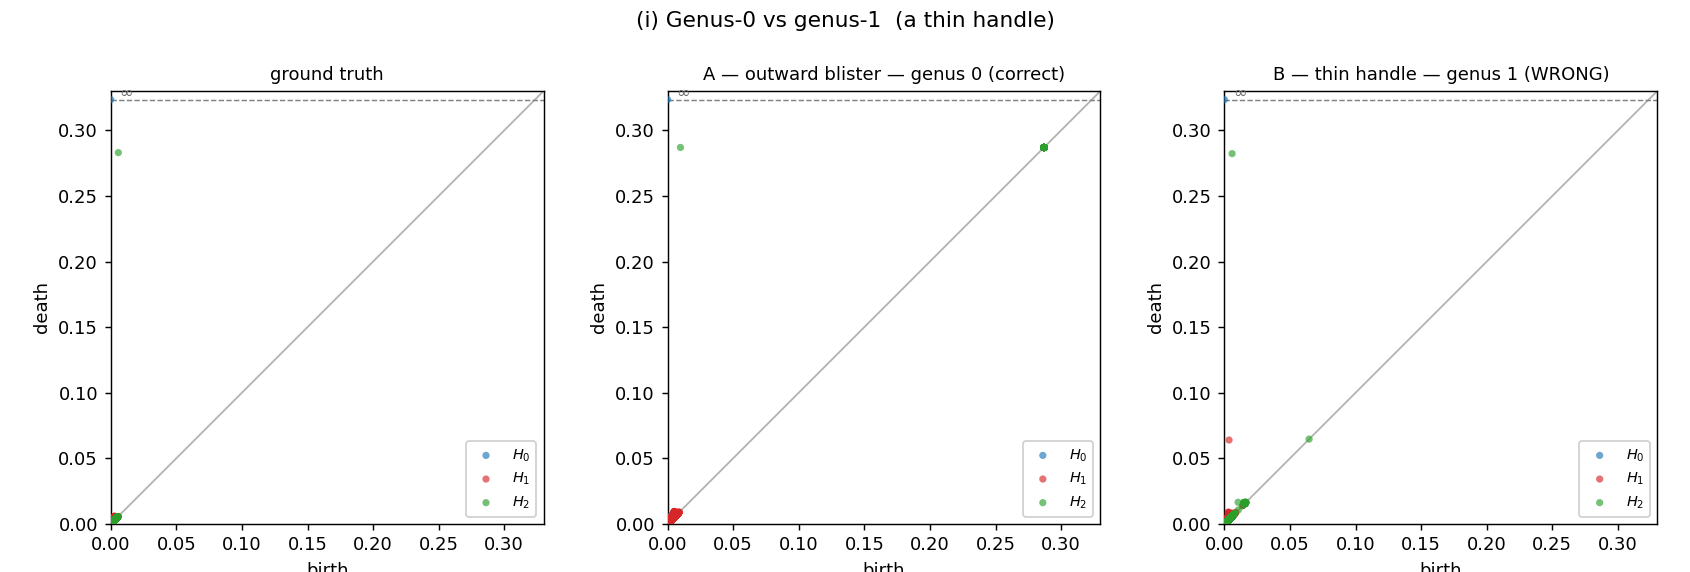
\includegraphics[width=0.32\linewidth]{pd_i_genus.png}\hfill
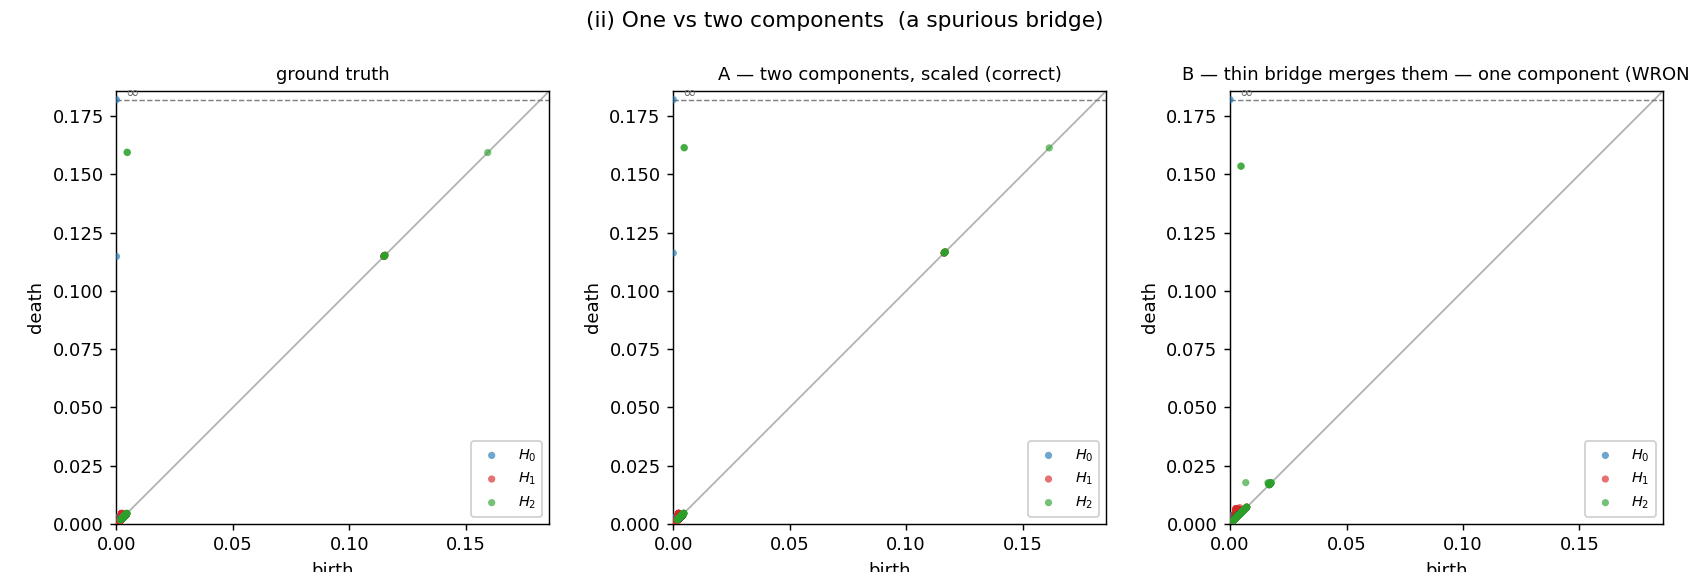
\includegraphics[width=0.32\linewidth]{pd_ii_components.png}\hfill
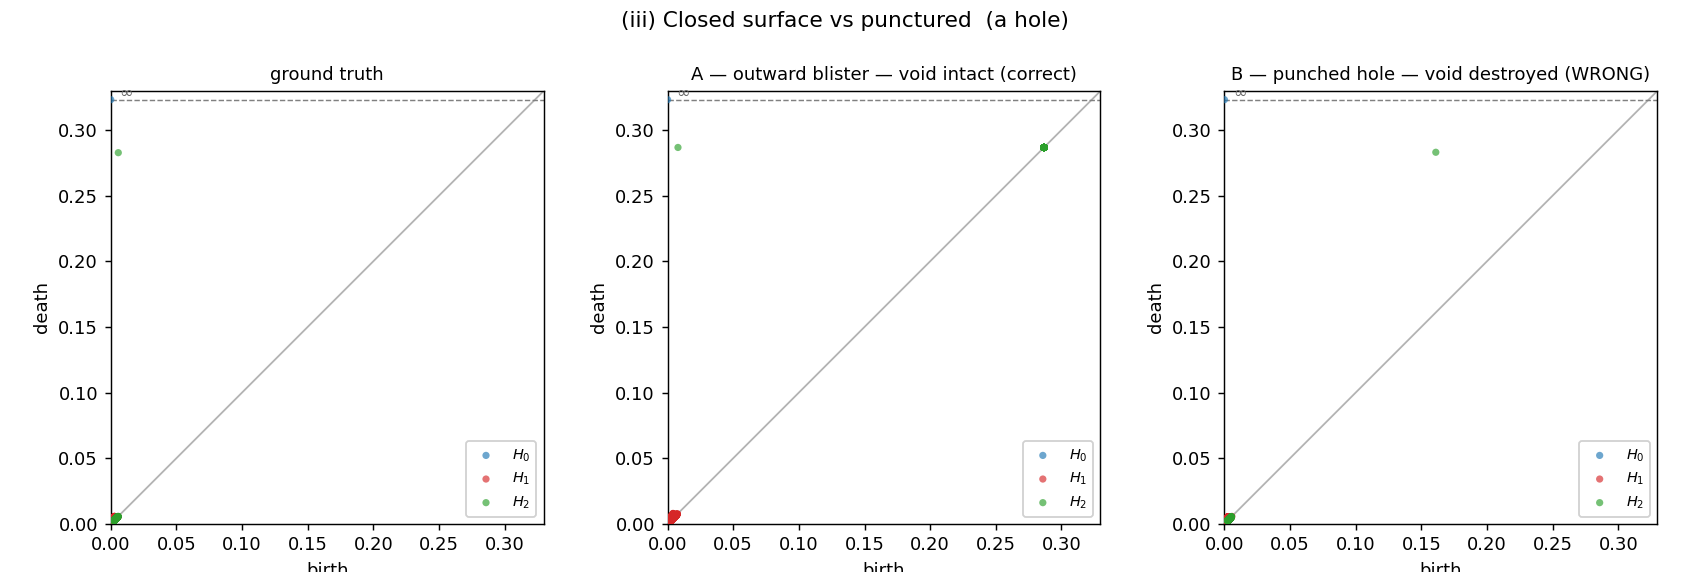
\includegraphics[width=0.32\linewidth]{pd_iii_void.png}
\caption{Persistence diagrams (GT / A / B) for the three blindness cases:
(i) genus, (ii) components, (iii) void.}
\label{fig:pd}
\end{figure}

A topological bias supplied only at initialization does not survive training:
the first resampling step removes it, so the final topology is independent of the
initial bias. The persistence-based stability series makes the gap
visible---Chamfer drifts smoothly while the bottleneck jumps when a spurious feature
becomes significant (Figure~\ref{fig:stability}).
% src(washout / stability series): D:\Project\CG-Soup-Topology\figures\summary.md,
% D:\Project\CG-Soup-Topology\figures\stability_series.csv
% TODO(human): if you want the exact step at which #sig-H1 flips 0->1, read it
% from stability_series.csv and state it.

\begin{figure}[h]
\centering
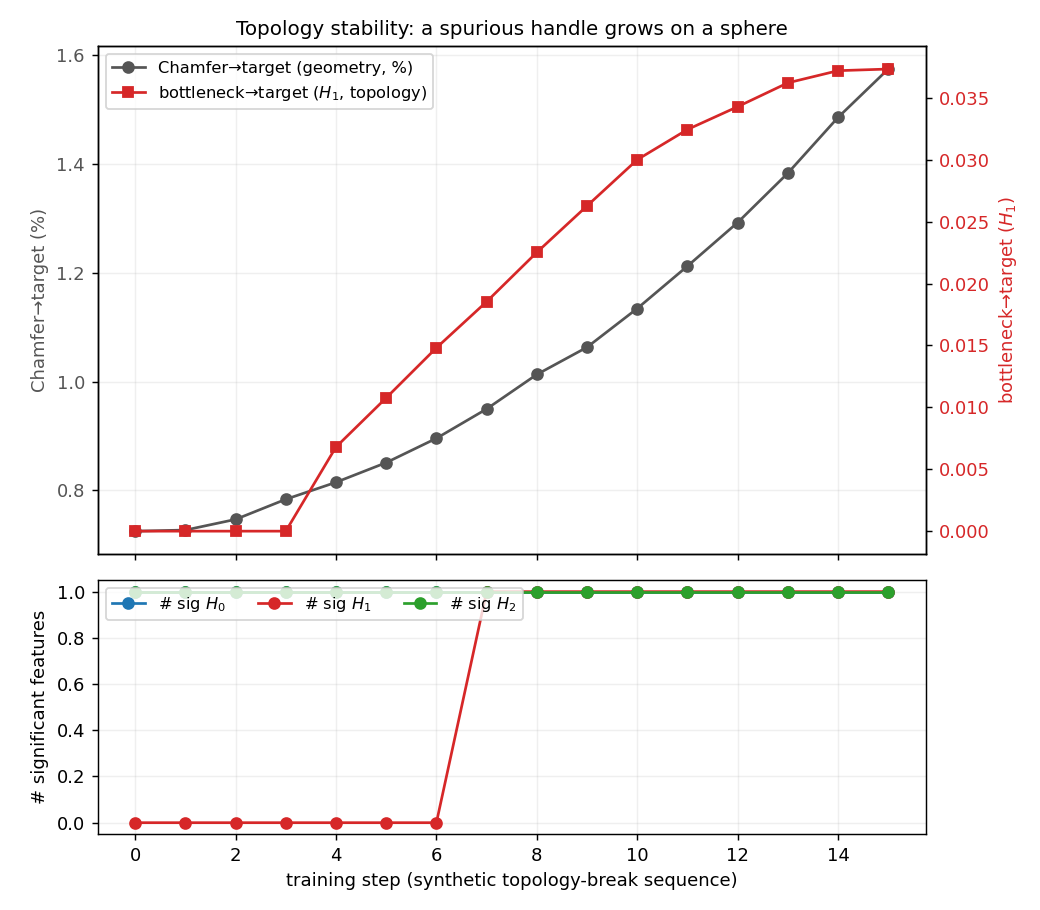
\includegraphics[width=0.7\linewidth]{stability_series.png}
\caption{Topology stability series: Chamfer (smooth) vs bottleneck-H1 (jumps when
a spurious handle becomes significant).}
\label{fig:stability}
\end{figure}

% ---- 5.2 Voids: width vs placement (2x2), one run: h2_unified, 5 seeds -------
\subsection{Voids (H2): mostly width, with a shape-dependent topological residual}
\label{sec:results-h2}

For voids, spreading the resampling prior helps substantially---a controlled 2$\times$2
over \emph{kernel width} (narrow $s{=}1$ vs.\ wide $s{=}3$) and \emph{placement}
(topological vs.\ non-topological; Table~\ref{tab:h2}) shows the gain is chiefly a
\emph{width} effect with a smaller, shape-dependent topological component.
\emph{Width:} at matched placement, widening cuts error by 15--33\% (topological
B4-vs-B2 by 18--33\%, non-topological B5-vs-B3 by 15--33\%), so both \emph{wide} priors
land far below both \emph{narrow} ones. (Not every wide-vs-narrow \emph{cross}-pair
clears 15\%---e.g.\ B5-vs-B2 is $\approx$9\% for the cylinder---so the range is stated
for matched-placement widening.) \emph{Placement:} the topological-placement benefit is
real but shape-dependent, clearest for the cylinder, where topology helps at
\emph{both} widths (narrow B2-vs-B3 by 7.8\%; wide B4-vs-B5 by $\approx$4.6$\sigma$);
for the sphere it is weak (narrow: a tie; wide: $\approx$2.2$\sigma$), and for the cube
absent (a tie at both widths). B4 is the best single condition at better-or-equal
geometry, but a width-matched non-topological control recovers most of its advantage,
so the void gain is chiefly width with a real but shape-dependent topological residual.
Init-time bias washes out (B1${\approx}$B0).
% src(all numbers this subsection): D:\Project\CG-Soup-for-Digital-Dentistry\output\synth\h2_unified\report\results.json

\begin{table}[h]
\centering
\resizebox{\textwidth}{!}{%
\begin{tabular}{lcccccc}
\toprule
 & \multicolumn{2}{c}{narrow ($s{=}1$)} & \multicolumn{2}{c}{wide ($s{=}3$)} & & \\
\cmidrule(lr){2-3}\cmidrule(lr){4-5}
target (H2) & B2 topo & B3 non-topo & \textbf{B4 topo} & B5 non-topo & B0 base & $\Delta$(B4$-$B5) \\
\midrule
sphere   & 0.0438 & 0.0440 & \textbf{0.0357} & 0.0374 & 0.0535 & $-0.0017$ (2.2$\sigma$) \\
cube     & 0.0409 & 0.0403 & \textbf{0.0273} & 0.0270 & 0.0579 & $+0.0003$ (tie) \\
cylinder & 0.0440 & 0.0477 & \textbf{0.0360} & 0.0402 & 0.0545 & $-0.0042$ (4.6$\sigma$) \\
\bottomrule
\end{tabular}}
\caption{Voids, one paired-seed run ($N{=}1200$, 5 seeds): bottleneck-to-target
(decisive dim, tail mean; lower better) in a width$\times$placement 2$\times$2.
At matched placement, \emph{widening} cuts error by 15--33\% (B4-vs-B2, B5-vs-B3);
\emph{placement} is a smaller, shape-dependent residual---the topological column beats
the non-topological one clearly for the cylinder (both widths), weakly for the sphere
(wide only), and not for the cube. $B0$ is the baseline; $B1{\approx}B0$ (init washout,
omitted).}
% src: h2_unified/report/results.json (bott_tail_mean; B4-B5 z from bott_tail_sd, 5 seeds)
\label{tab:h2}
\end{table}

\begin{figure}[h]
\centering
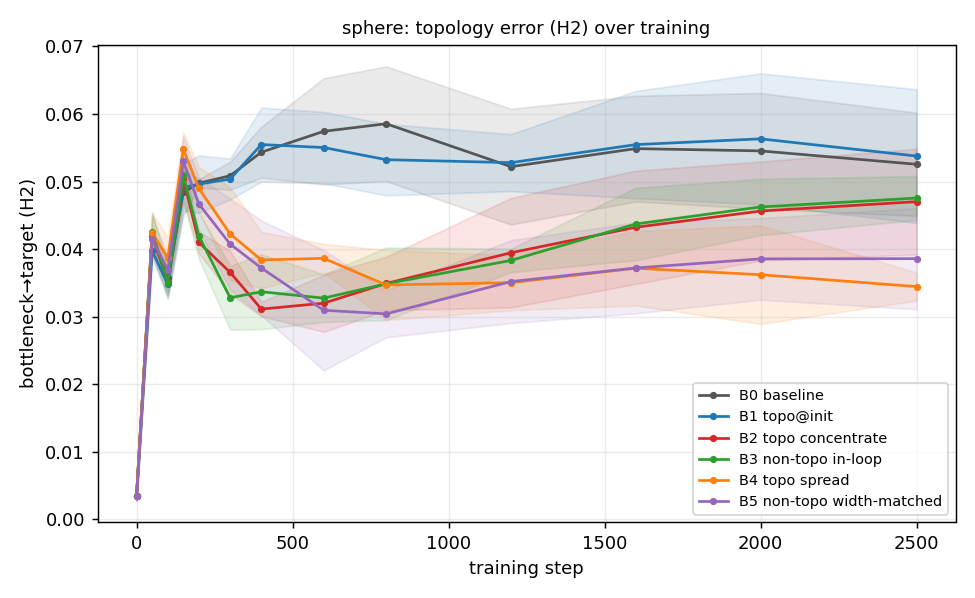
\includegraphics[width=0.32\linewidth]{sphere_bottleneck.png}\hfill
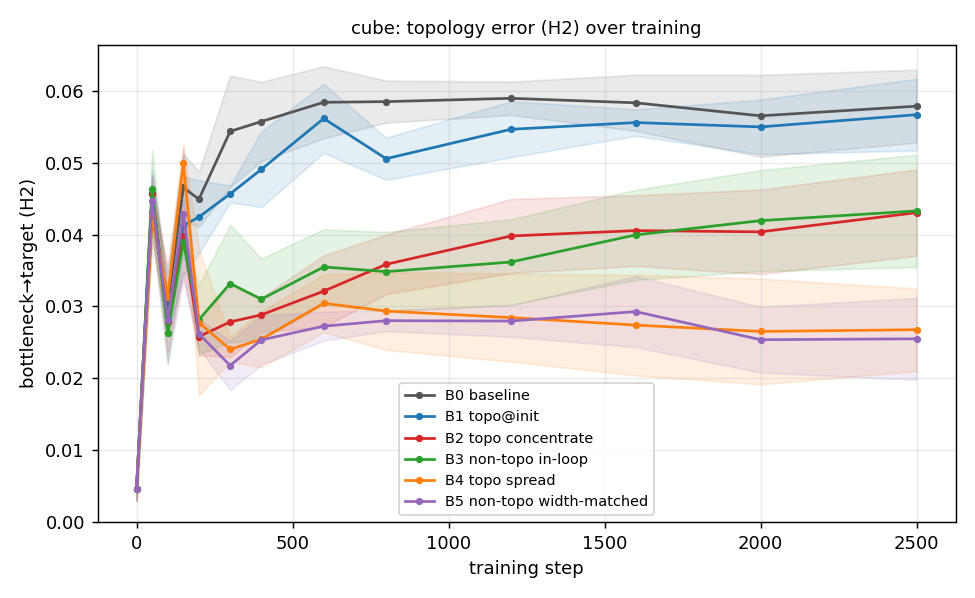
\includegraphics[width=0.32\linewidth]{cube_bottleneck.png}\hfill
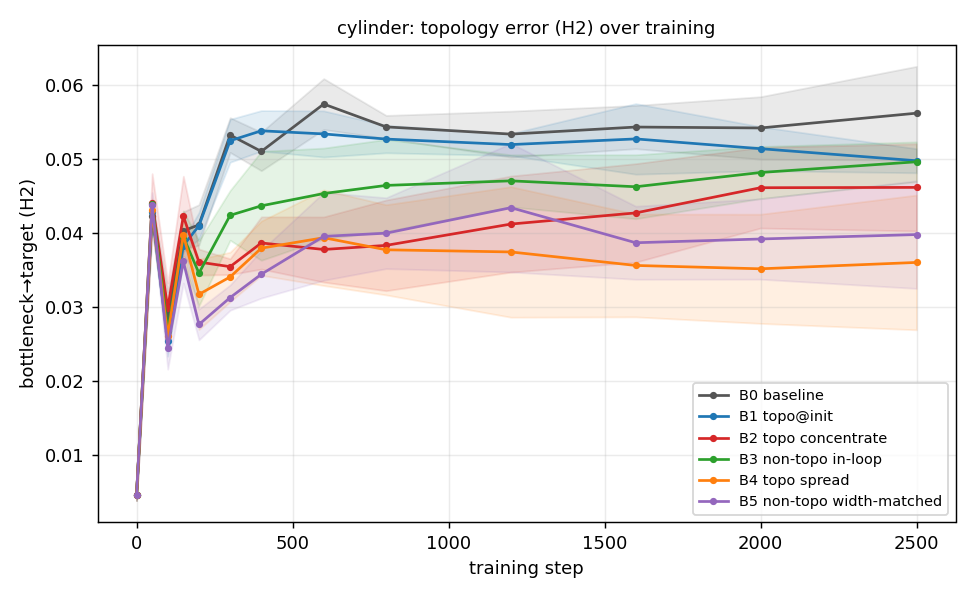
\includegraphics[width=0.32\linewidth]{cylinder_bottleneck.png}
\caption{Bottleneck-to-target over training for the three voids (conditions B0--B5):
the two \emph{wide} priors (B4 topological, B5 non-topological) track well below the
two \emph{narrow} priors (B2, B3), and B4/B5 nearly coincide---width, not topology,
is the driver. Geometry parity: Figure~\ref{fig:sphere-geom}.}
\label{fig:h2}
\end{figure}

\begin{figure}[h]
\centering
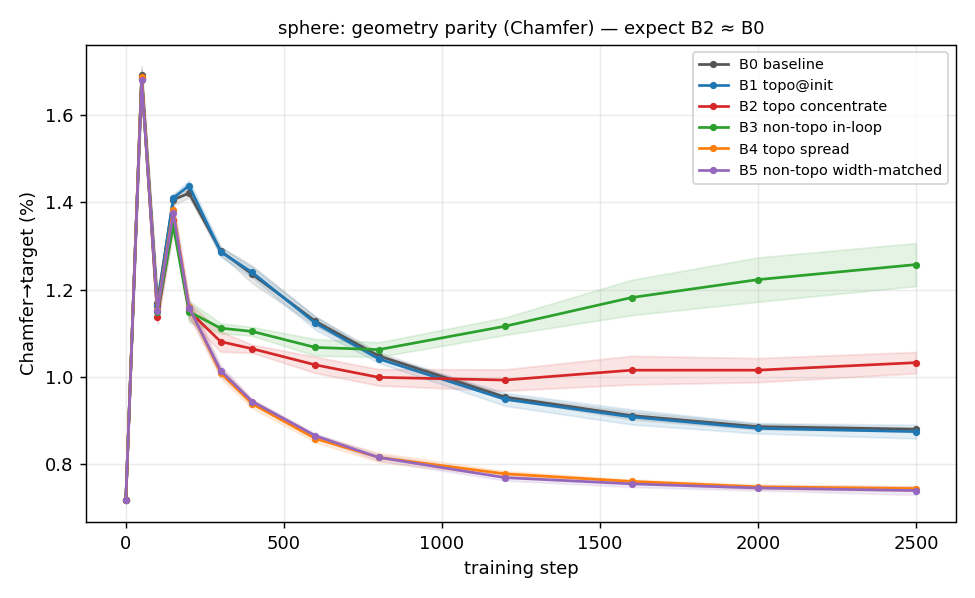
\includegraphics[width=0.55\linewidth]{sphere_geometry.png}
\caption{Sphere geometry (Chamfer): B4 (spread) sits at or below baseline, so the
topological gain is not bought with geometry.}
\label{fig:sphere-geom}
\end{figure}

Whether this ``spread beats concentrate'' ordering is special to voids or holds
across feature dimensions is the subject of Section~\ref{sec:results-crossover}.

% ---- 5.3 Crossover across dimensions (H2 rows from Table 1; low-dim from crossover) --
\subsection{Does the optimal prior flip with dimension?}
\label{sec:results-crossover}

Section~\ref{sec:results-h2} shows spread beats concentrate for voids. Does a
low-dimensional feature instead prefer concentration---a \emph{dimensional
crossover}? We compare the concentrated (B2) and spread (B4) priors---identical but
for the width scale---in each shape's decisive dimension, at a per-class
\emph{headroom} budget, and track the signed difference
$\Delta=\text{bottleneck}(\text{B4})-\text{bottleneck}(\text{B2})$
(Table~\ref{tab:crossover}); a crossover would show $\Delta$ change sign with
dimension. We add a genus-2 \texttt{double\_torus} ($b_1{=}4$) and
\texttt{three\_spheres} ($b_0{=}3$).

\begin{table}[h]
\centering
\begin{tabular}{llcccc}
\toprule
target & dim & $N$ & B2 concentrate & B4 spread & $\Delta=$B4$-$B2 \\
\midrule
sphere         & H2 & 1200 & 0.0438 & 0.0357 & $-0.0081$ \\
cube           & H2 & 1200 & 0.0409 & 0.0273 & $-0.0136$ \\
cylinder       & H2 & 1200 & 0.0440 & 0.0360 & $-0.0080$ \\
torus          & H1 &  700 & 0.0425 & 0.0316 & $-0.0109$ \\
two\_spheres   & H0 &  700 & 0.0059 & 0.0057 & $-0.0002$ \\
three\_spheres & H0 &  700 & 0.0062 & 0.0053 & $-0.0009$ \\
double\_torus  & H1 & 2000 & \multicolumn{3}{c}{inconclusive (bottleneck pinned; see text)} \\
\bottomrule
\end{tabular}
\caption{Concentrate vs.\ spread across feature dimensions: $\Delta\le 0$
\emph{everywhere}, so there is no sign flip and no crossover---spread is at least as
good as concentrating at every dimension, and strictly better for voids and the
torus. The H2 rows are the paired-seed run of Table~\ref{tab:h2} (h2\_unified, 5
seeds); the low-dimensional rows are the crossover run (torus 5 seeds, others 3).
Each row is internally consistent (one run per shape).}
% src(H2 rows): D:\Project\CG-Soup-for-Digital-Dentistry\output\synth\h2_unified\report\results.json
% src(low-dim rows): D:\Project\CG-Soup-for-Digital-Dentistry\output\synth\crossover\crossover_report\results.json
\label{tab:crossover}
\end{table}

\paragraph{No crossover; spread wins or ties everywhere.} $\Delta=$B4$-$B2 (spread
minus concentrate, both \emph{topological}) is clearly negative for voids and the torus
(spread better) and only marginally negative for the two H0 shapes---within noise of the
non-topological control, i.e.\ a null. Nowhere does concentrating win, so the optimal
spatial prior does not flip with dimension. Because this $\Delta$ holds placement fixed
(both priors topological), it isolates the effect of \emph{width}; whether the loop
spread-win is \emph{topological} needs the non-topological arm, which we add for the
torus next (Table~\ref{tab:torus2x2}).

\paragraph{On the loop, width drives the gain; topological placement does not.} A
width$\times$placement 2$\times$2 on the torus (Table~\ref{tab:torus2x2}), mirroring the
void analysis, decomposes the spread-win. \emph{Width} helps massively at either
placement: widening drops the bottleneck $26\%$ for the topological pair (B2$\to$B4) and
$33\%$ for the non-topological pair (B3$\to$B5), putting both \emph{wide} cells far below
both \emph{narrow} ones. \emph{Placement}, by contrast, gives no benefit on the
loop---at both widths the \emph{non-topological} prior is better: narrow B3 $0.0397 <$ B2
$0.0425$ ($7.6\sigma$) and wide B5 $0.0267 <$ B4 $0.0316$ ($3.25\sigma$), so the best
torus condition is a \emph{wide non-topological} prior. The only distinctly topological
effect is a harmful one: at this budget only the narrow-topological prior (B2) inflates
significant-H1 into phantom handles ($4.4$ vs.\ a true $2$; B3, B4, and B5 all hold
$2.0$), the concentrate backfire of Section~\ref{sec:mechanism}. So on the torus, as on
the voids, \emph{width} drives the gain---but here topological placement is a small cost,
not a small residual.
% src(torus B0/B2/B3/B4/B5 bottleneck + #sig, N=700, 5 seeds): D:\Project\CG-Soup-for-Digital-Dentistry\output\synth\crossover\report\results.json

\begin{table}[h]
\centering
\begin{tabular}{lccccc}
\toprule
 & \multicolumn{2}{c}{narrow ($s{=}1$)} & \multicolumn{2}{c}{wide ($s{=}3$)} & \\
\cmidrule(lr){2-3}\cmidrule(lr){4-5}
torus (H1), $N{=}700$ & B2 topo & B3 non-topo & B4 topo & \textbf{B5 non-topo} & B0 \\
\midrule
bottleneck (tail mean) & 0.0425 & 0.0397 & 0.0316 & \textbf{0.0267} & 0.0409 \\
significant-H1 (true $2$) & 4.4 & 2.0 & 2.0 & 2.0 & 2.0 \\
\bottomrule
\end{tabular}
\caption{Torus width$\times$placement 2$\times$2 (5 paired seeds, $N{=}700$), mirroring
Table~\ref{tab:h2} for a loop. \emph{Width} helps at either placement (both wide cells
far below both narrow); at matched \emph{placement} the \emph{non-topological} prior is
better at both widths (narrow $7.6\sigma$, wide $3.25\sigma$), so the loop spread-win is
a width effect. Topological placement's only distinct effect is harmful: the
narrow-topological B2 alone inflates significant-H1 into phantom handles.}
% src: crossover/report/results.json (bott_tail_mean, final_nsig; z from bott_tail_sd, 5 seeds)
\label{tab:torus2x2}
\end{table}

\paragraph{Components are a null.} For \texttt{two\_spheres} and
\texttt{three\_spheres} neither topological prior beats the non-topological control:
component correctness is governed by the \emph{absence} of geometry in the
inter-component gap, which a placement prior does not control
(Section~\ref{sec:mechanism}).
% src: crossover/crossover_report/results.json

\paragraph{Multi-loop genus-2: inconclusive.} On \texttt{double\_torus} the
decisive-dimension bottleneck is identical across all conditions (pinned at
$0.0264$) and the soup recovers only 2 of the 4 loops at every budget tried, so
this stress test does not discriminate; we report it as inconclusive rather than
support, and flag a higher-resolution re-run as future work.
% src(double_torus pinned 0.0264, #sig 2): crossover/crossover_report/results.json

\begin{figure}[h]
\centering
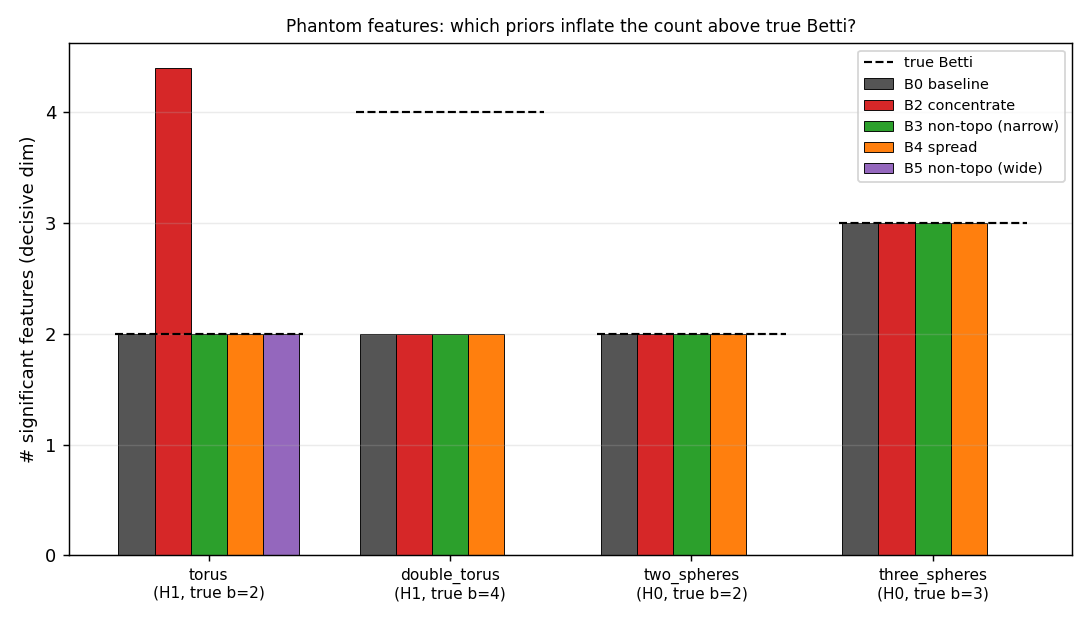
\includegraphics[width=0.6\linewidth]{phantom.png}
\caption{Significant-feature count vs.\ true Betti (low-dimensional shapes):
concentrate (B2) inflates the torus H1 count (phantom handles), while spread (B4)
\emph{and} both non-topological priors (narrow B3, wide B5; Table~\ref{tab:torus2x2})
hold the true value---so the inflation is specific to the narrow-\emph{topological}
prior; the H0 shapes are unaffected.}
\label{fig:phantom2}
\end{figure}

% ===== 6. Mechanism / discussion ============================================
% Aligned to the paper's thesis: a SPREAD prior wins at every dimension; what
% depends on dimension is the HARM from concentrating. No spliced numbers here ---
% H2 magnitudes live in their tables (Sec 5.2 / 5.3); the torus backfire cites the
% crossover (Sec 5.3) for N=700 and an INDEPENDENT budget sweep (Fig) at N=400.
% ISSUE-1 (cross-run splice) is a separate, pending data decision.
\section{Why spreading wins, and why concentration's harm depends on dimension}
\label{sec:mechanism}

\paragraph{What the importance scale actually varies.}
A feature's death simplex marks \emph{where} its topology is fragile, but the
feature's support is larger---the bounding shell of a void, the whole tube of a
handle. For the compact targets used here the feature's death scale is of order the
shape size, so even the concentrated field ($s{=}1$) already overlaps most of the
surface. The scale $s$ therefore varies the \emph{peakedness} of the field---and
hence the differential protection the keep-map applies to feature geometry---far
more than its literal spatial coverage. ``Spreading'' here means ``protect the
feature's whole support evenly,'' not ``reach more of the surface.''
% src(limited dynamic range / peakedness): PHASE2B_CROSSOVER.md (Caveats)

\paragraph{Voids: spreading (width) helps; topological placement is a small residual.}
An enclosed void is destroyed by a hole \emph{anywhere} on the 2-manifold shell that
bounds it, so the void's support---the geometry whose failure collapses it---is the
\emph{entire} shell, which for a compact shape is essentially the whole surface. As the
peakedness caveat above notes, even the concentrated field ($s{=}1$) already overlaps
most of that surface, so \emph{any} wide field---topological or not---approximately
spreads over the void's support. The single principle ``spread over the support''
therefore predicts the void effect should look width-driven, with topological placement
only a residual---and it is: a width-matched non-topological control (B5) recovers most
of the spread prior's gain (Section~\ref{sec:results-h2}). That residual---placing the
wide prior at the void locus (B4) rather than at random (B5)---should track how
\emph{non-uniform} the bounding shell is, and it does: largest for the cylinder (flat
caps and a curved side; $\approx$4.6$\sigma$), smaller for the near-uniform sphere
($\approx$2.2$\sigma$), and absent for the cube (a tie).
% src(B4-B5 residual + sigma): D:\Project\CG-Soup-for-Digital-Dentistry\output\synth\h2_unified\report\results.json

\paragraph{The harm of concentrating, and why it scales with dimension.}
What \emph{does} depend on dimension is the damage a concentrating prior does, and
it is governed by how readily over-tessellating a \emph{single} locus
\emph{fabricates a spurious feature of the same dimension}:
\begin{itemize}
  \item \textbf{Loops (1-D): catastrophic, and here placement matters.} A loop's
  support is a thin tube, far smaller than the surface, so a \emph{narrow} prior cannot
  spread along it and over-tessellates it into phantom handles---the significant-H1
  count rises above the true value and the bottleneck worsens \emph{below baseline}
  (Section~\ref{sec:results-crossover}). At the headroom budget this backfire is
  \emph{narrow-topological}-specific: only the narrow-topological prior inflates the
  count ($N{=}700$: B2 $4.4$ vs.\ narrow-random B3 $2.0$; Table~\ref{tab:torus2x2}).
  Only under severe budget starvation does narrowness alone begin to over-tessellate a
  random prior too ($N{=}400$, 3 seeds: B2 ${\approx}\,7.7$, B3 ${\approx}\,5.7$, true
  value $2$; Figure~\ref{fig:phantom}). Either way the cure is \emph{width}: a wide
  prior, topological or not, recovers the true count.
  % src(N=700 #sig B2 4.4/B3 2.0: crossover/report; N=400 B2 7.67/B3 5.67: tight_N400/report): D:\Project\CG-Soup-for-Digital-Dentistry\output\synth\crossover\report\results.json
  \item \textbf{Voids (2-D): mild.} Over-tessellating one shell patch cannot
  \emph{create} a second enclosed void, so concentrating fabricates no spurious H2;
  it merely under-protects the rest of the shell---an incomplete-protection shortfall
  behind spreading, never worse than baseline.
  \item \textbf{Components (0-D): none.} A component boundary is defined by the
  \emph{absence} of geometry between shells; no placement of triangles on the shells
  adds or removes a component, so a placement prior has no purchase and the result
  is a null---neither topological prior beats the non-topological control
  (Section~\ref{sec:results-h2}).
\end{itemize}

\begin{figure}[h]
\centering
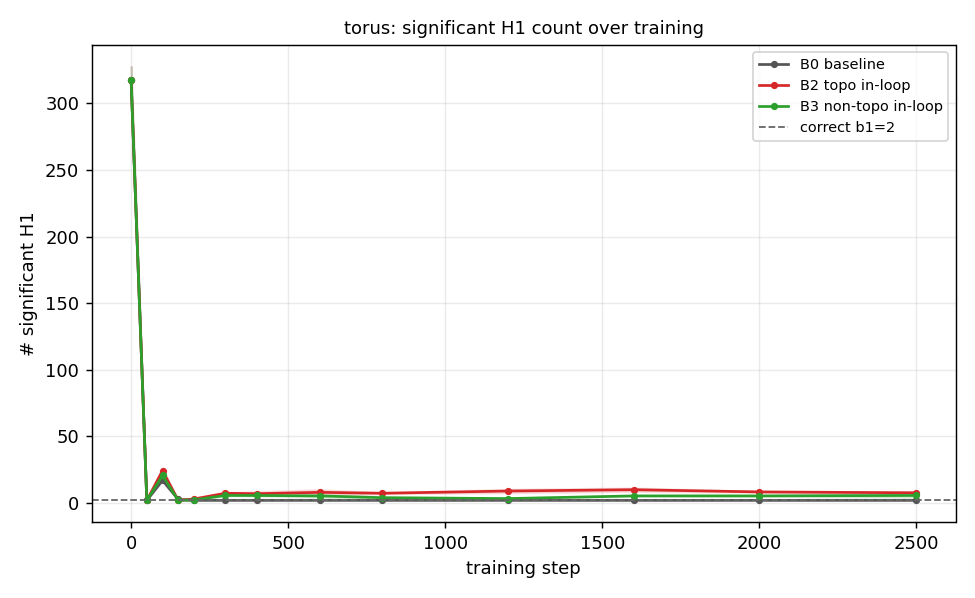
\includegraphics[width=0.6\linewidth]{torus_betti_N400.png}
\caption{Independent budget sweep, torus at the tight budget $N{=}400$: \emph{both}
narrow priors inflate the significant-H1 count above the true value (phantom
handles)---the narrow-topological B2 more than the narrow-random B3---while the baseline
recovers the correct count. The over-tessellation is a narrowness effect, worsened by
topological placement.}
% src: D:\Project\CG-Soup-for-Digital-Dentistry\output\synth\tight_N400\report\torus_betti.png
\label{fig:phantom}
\end{figure}

\paragraph{Interpretation: one principle, two observable regimes.}
A single principle organizes all three cases---spread importance over the feature's
\emph{support}, not its localized death simplex---and, together with the peakedness
caveat, it predicts \emph{why} voids look width-driven while loops look
narrowness-driven: the difference is how much of the surface the support occupies. A
void's support is the whole bounding shell ($\approx$ the entire compact surface), so
any wide field already spreads over it and topological placement is only a residual
(Section~\ref{sec:results-h2}). A loop's support is a thin tube, far smaller than the
surface: a wide field does not specifically spread along that tube, and a \emph{narrow}
field over-tessellates it into phantom handles---so here narrowness is harmful and the
wide (spread) prior recovers the correct topology (Section~\ref{sec:results-crossover}).
The optimal prior is thus spread at every dimension (no crossover); only the observable
signature---and the harm from being narrow---depends on the support's extent. The
genus-2 multi-loop case did not resolve at feasible budgets and is reported as
inconclusive.
% src(spread > concentrate at every dim; H0 null; double_torus inconclusive): crossover/crossover_report/results.json

% ===== 7. Limitations & future work (DRAFTABLE) =============================
\section{Limitations and future work}
\label{sec:limitations}

\paragraph{Synthetic targets.}
All experiments use analytic shapes rendered into multi-view scenes, chosen so
the ground-truth surface and its Betti numbers are exact and so geometry can be
held fixed while topology varies---the control that makes the blindness result
and the topological-vs-non-topological comparison clean. The cost is external
validity: we do not yet demonstrate the method on captured or noisy real scenes,
where the target persistence diagram itself must be estimated.
% TODO(human): if you run any real/captured scene, add it; otherwise keep this honest.

\paragraph{Non-determinism of the optimizer.}
The CUDA rasterizer's gradient atomics make vertex positions non-reproducible
run-to-run; resampling structure ($F$) is deterministic but vertex positions
($V$) are not, so single-run differences can include a few drifting triangles. We
mitigate with paired seeds and seed-averaging and a soup-sampled topology metric,
but absolute numbers carry this run-to-run variance.
% src(determinism caveat): D:\Project\CG-Soup-Topology\PHASE2_STATUS.md

\paragraph{What the spread scale varies (limited dynamic range).}
For the compact targets used here, topological death scales are of order the shape
size, so even the concentrated field ($s{=}1$) already overlaps most of the surface.
The scale $s$ therefore controls the \emph{peakedness} of the importance field---and
thus the differential protection applied by the keep-map---rather than its literal
spatial coverage; our claims about ``spreading'' should be read in that sense.
Characterizing the effect on targets whose features are small relative to the shape,
where coverage and peakedness decouple, is left to future work.
% src(limited dynamic range / peakedness): PHASE2B_CROSSOVER.md (Caveats)

\paragraph{Width vs.\ topological placement.}
The void gain is primarily a kernel-width effect: a width-matched non-topological
control recovers most of it, and the residual attributable to topological placement
is small and shape-dependent---clear for the cylinder, modest for the sphere, absent
for the cube (Section~\ref{sec:results-h2}). Establishing that residual robustly, and
whether it grows for targets with finer or off-centre voids, would need more shapes
and seeds.
% src(width-matched control B5): D:\Project\CG-Soup-for-Digital-Dentistry\output\synth\h2_unified\report\results.json

\paragraph{Precomputed, non-differentiable prior.}
The importance field is distilled once from the target and is \emph{not}
differentiated through; the method biases sampling, it does not flow a topological
gradient. Making persistent homology differentiable so the topological signal can
backpropagate into vertex positions---rather than only steer resampling---is the
natural next phase, building on existing differentiable-persistence
machinery~\cite{gabrielsson2020topologylayer,carriere2021optimizing,poulenard2018shapematching}.
% src(scope: precomputed field, no differentiable PH): methods/topo_importance.py header

\paragraph{Resolving multi-loop / genus-2 targets.}
Our genus-2 \texttt{double\_torus} stress test was inconclusive: at every feasible
budget the soup recovered only 2 of its 4 loops and the decisive-dimension
bottleneck did not discriminate between conditions
(Section~\ref{sec:results-crossover}). Strengthening the spread-vs-concentrate
finding on a richer multi-loop target needs a higher-resolution or longer-schedule
re-run, which we leave to future work.
% src(double_torus inconclusive): D:\Project\CG-Soup-for-Digital-Dentistry\output\synth\crossover\crossover_report\results.json


\bibliographystyle{plainnat}
\bibliography{refs}

\end{document}
